% ------------------------------------------------------------------------------
% section 03
% ------------------------------------------------------------------------------
\newpage
\section{Questions 3}
\label{cha:q3}

\subsection[Q3-a]{Consider the numerical variables in the data set and find the best SIMPLE linear regression model to predict the prices. Test the assumptions and use transformations if it is required. Explain why the model you find is the best simple linear regression model and interpret the model coefficients.}

\begin{figure}[htbp]
    \centering
    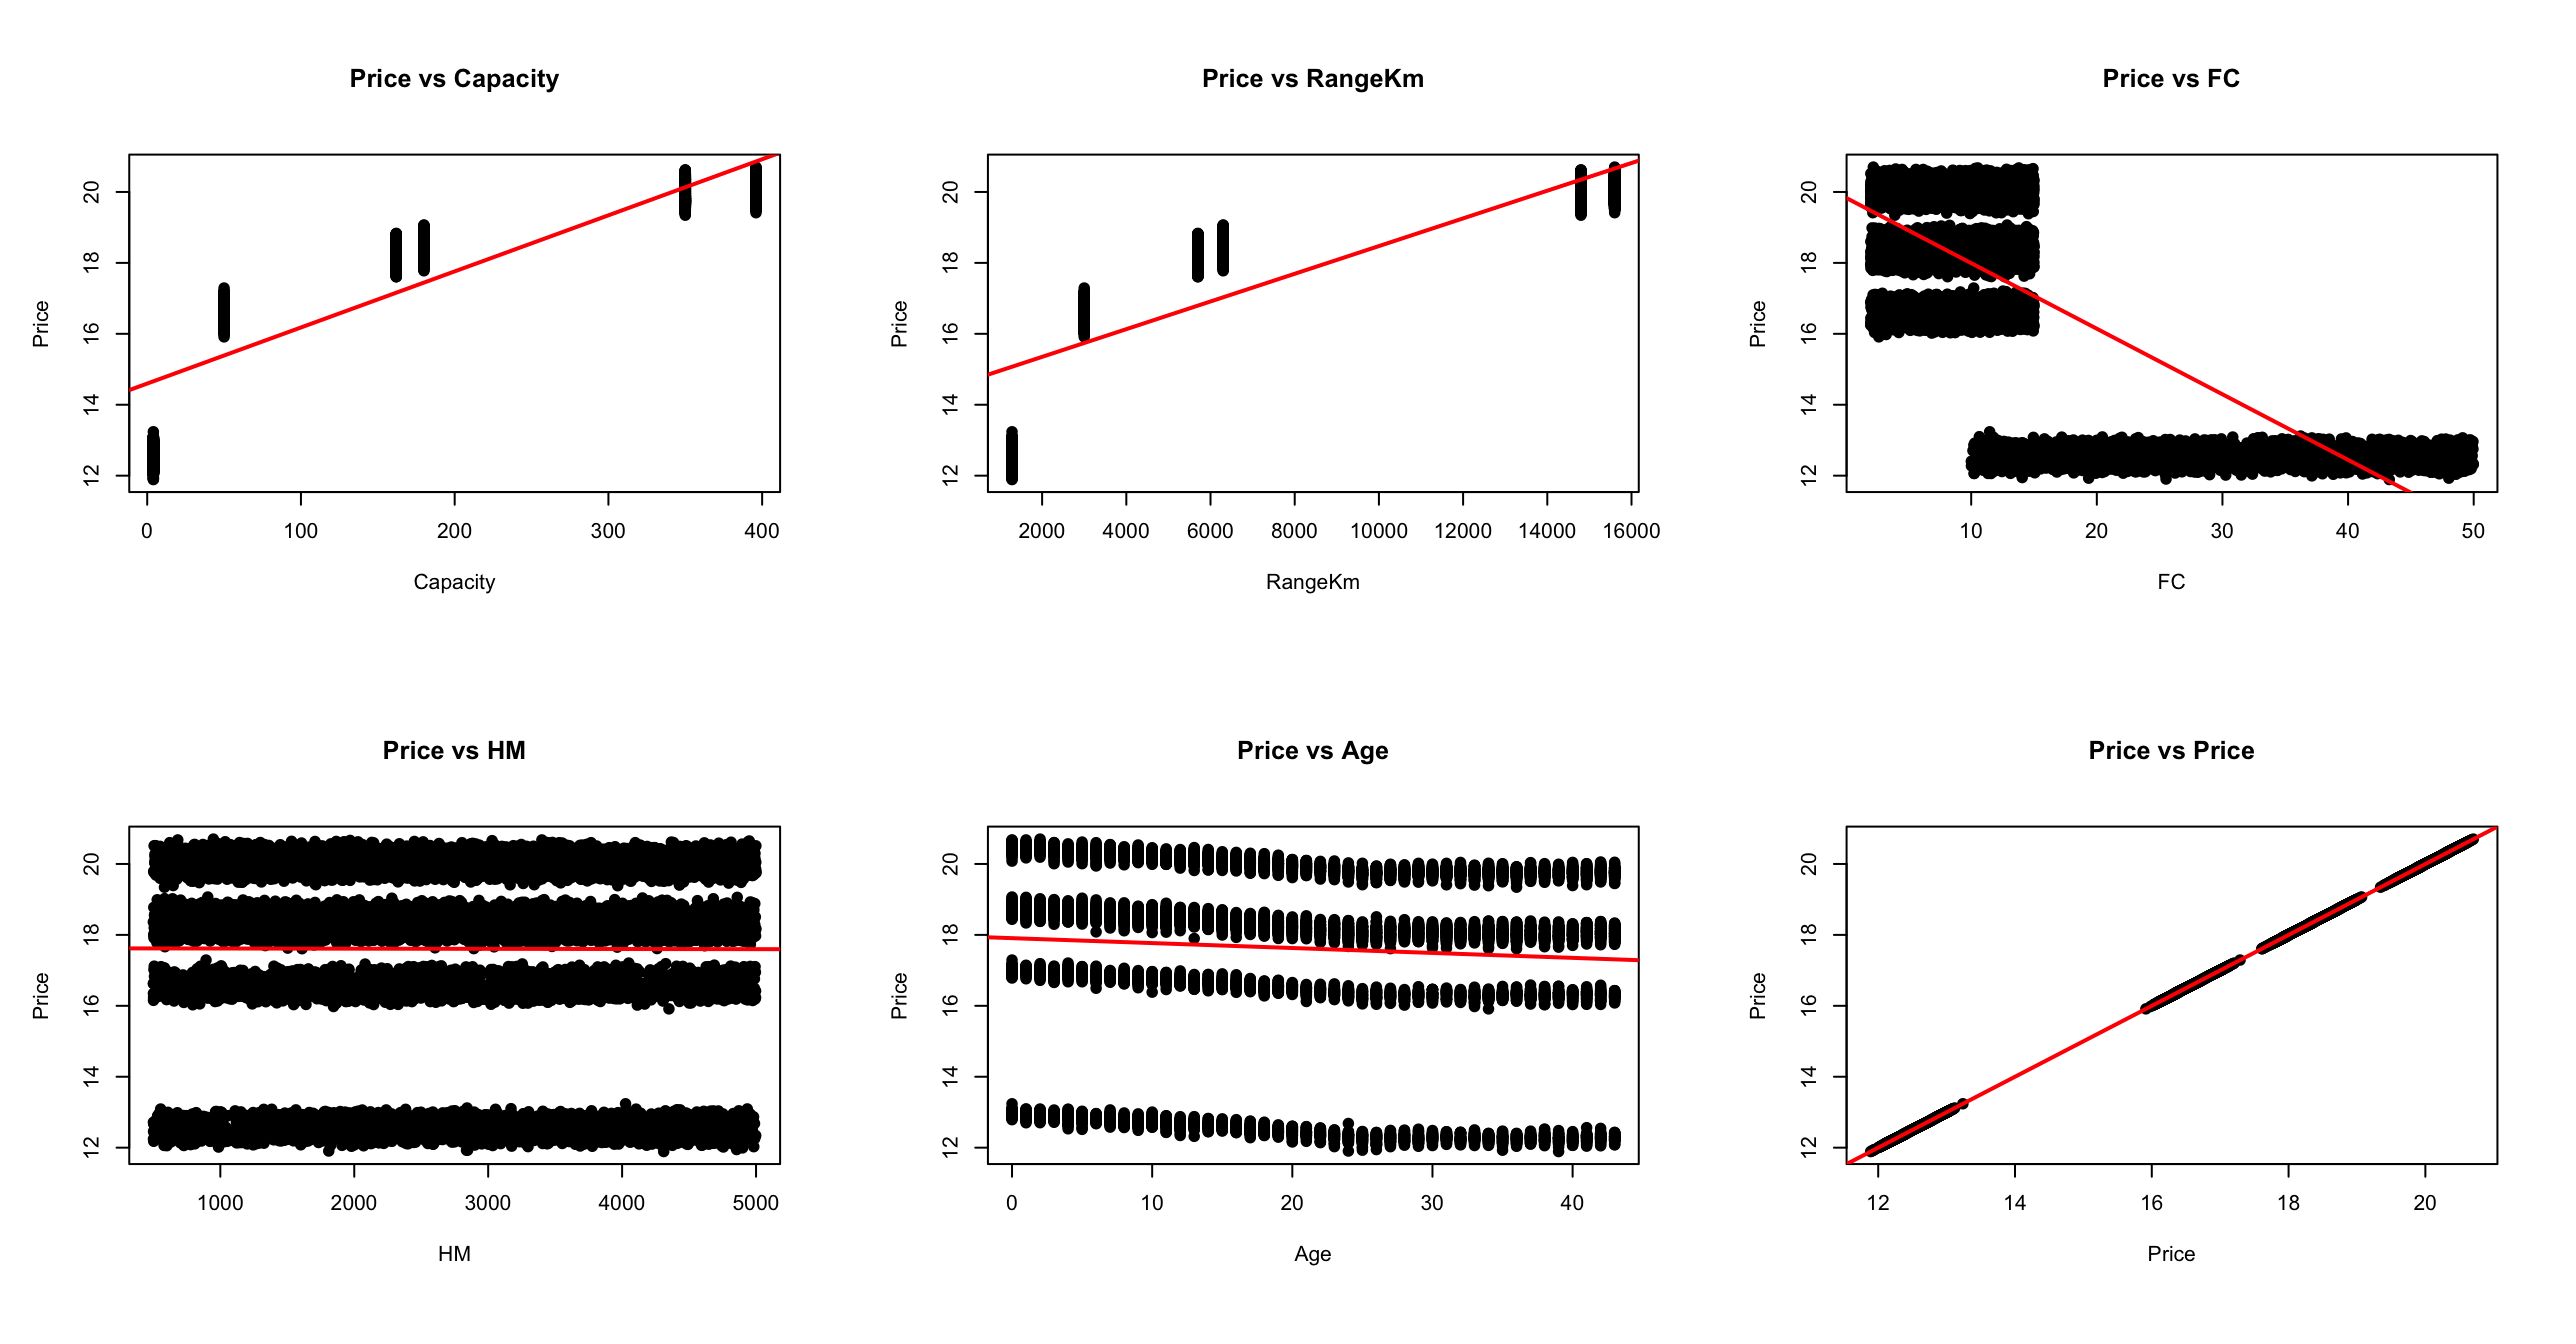
\includegraphics[width=\figsizetext]{Q3/01-price-plots.png}
    \caption{Price plots analysis}
    \label{fig:q3_01}
\end{figure}

According to plot analysis (figure \ref{fig:q3_01}), we selected the variables \texttt{Capacity}, \texttt{RangeKm}, and \texttt{FC} (Fuel Consumption) as the best candidates for the linear model because they show the most linear relationship with \texttt{Price}. A $\log()$ transformation was applied to \texttt{Price} to normalize its distribution.

The correlation matrix confirmed that \texttt{Capacity}, \texttt{RangeKm}, and \texttt{FuelConsumption} are the top 3 numerical variables with the highest correlation to \texttt{Price}.

\begin{figure}[htbp]
    \centering
    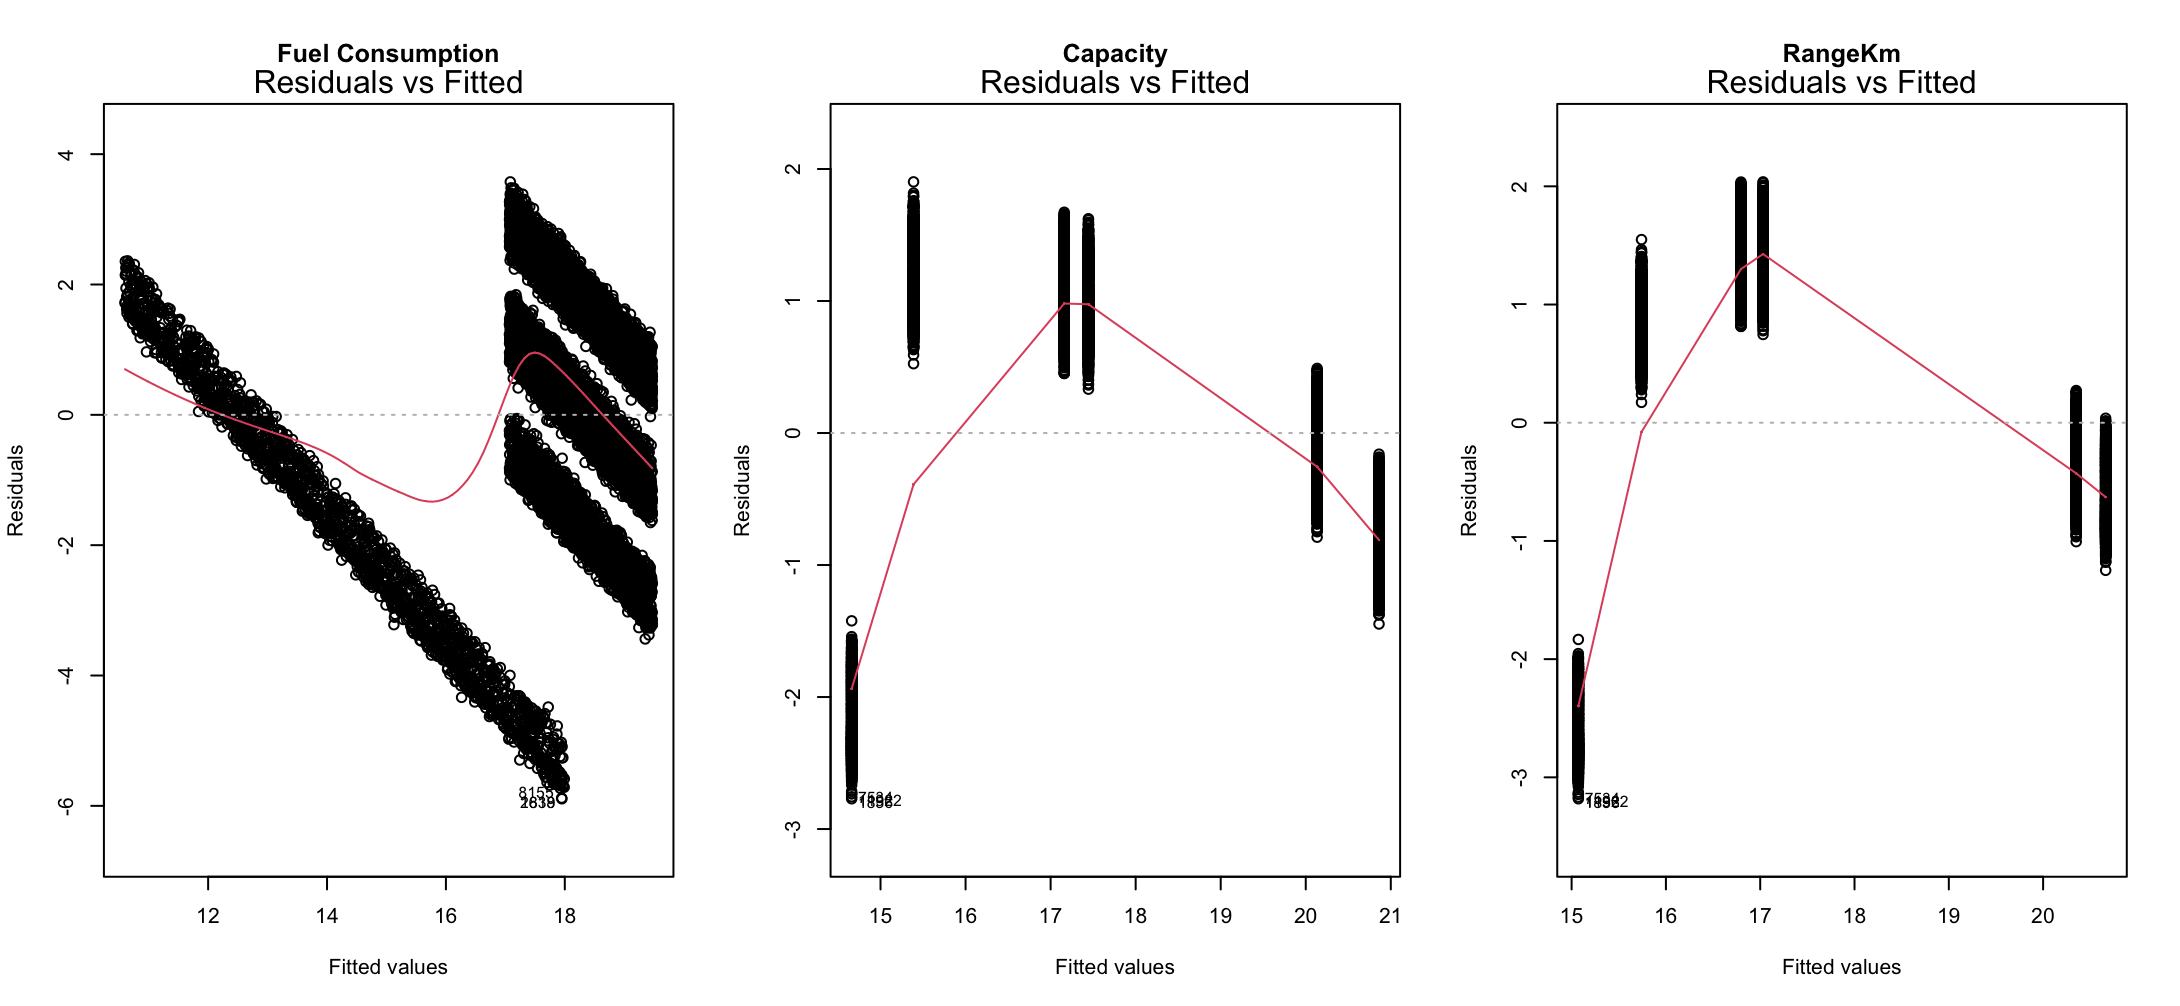
\includegraphics[width=\figsizetext]{Q3/02-plot-residual-vs-fitted.png}
    \caption{Residual vs Fitted plot}
    \label{fig:q3_02}
\end{figure}

The Residual vs Fitted plots (figure \ref{fig:q3_02}) suggested that the model may need a quadratic term. After comparing \texttt{Capacity} vs \texttt{RangeKm} using a quadratic term (figure \ref{fig:q3_02_1}), the ANOVA shows that \texttt{RangeKm} + $\texttt{RangeKm}^2$ yields the lowest RSS results.

\begin{figure}[htbp]
    \centering
    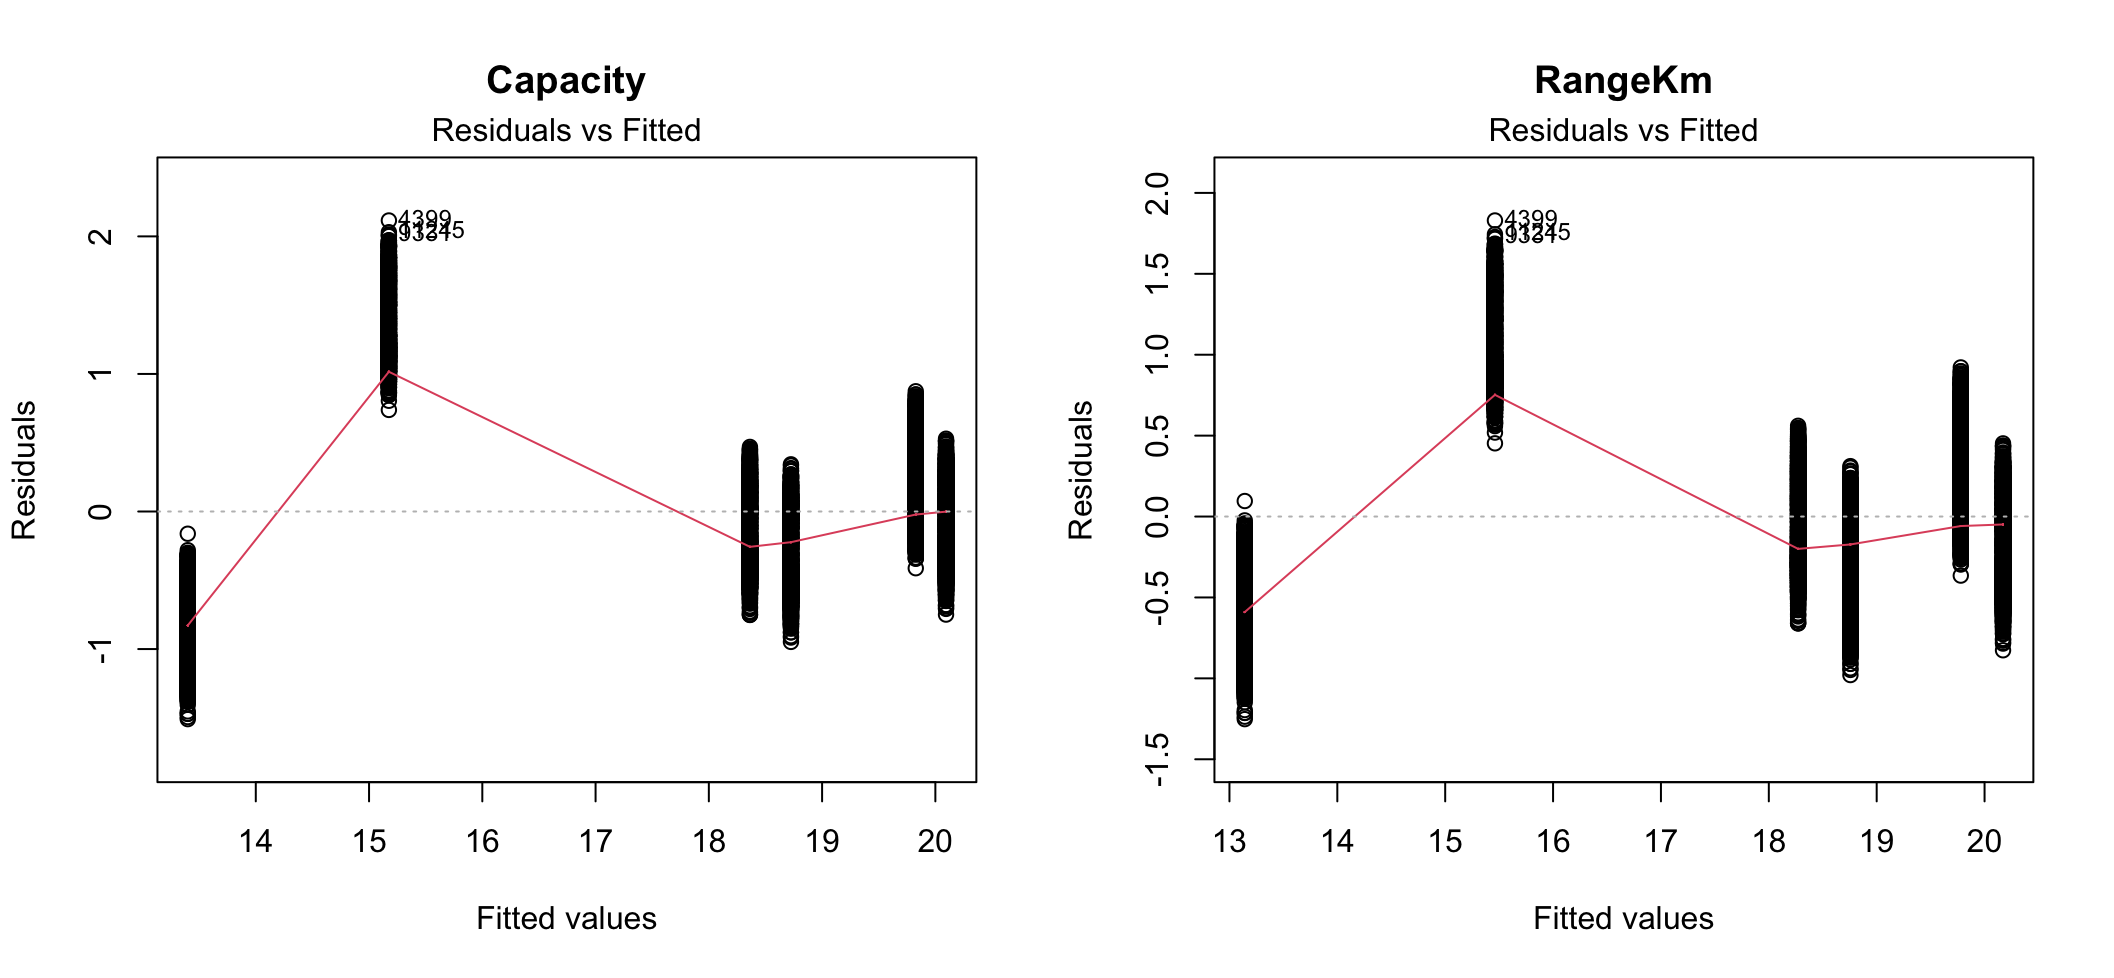
\includegraphics[width=\figsizetext]{Q3/02.1-plot-res-vs-fitted.png}
    \caption{Residual vs Fitted plot (Quadratic term)}
    \label{fig:q3_02_1}
\end{figure}

The new model with the quadratic term shows better residuals.

\subsubsection*{Regression assumptions analysis}

\begin{figure}[htbp]
    \centering
    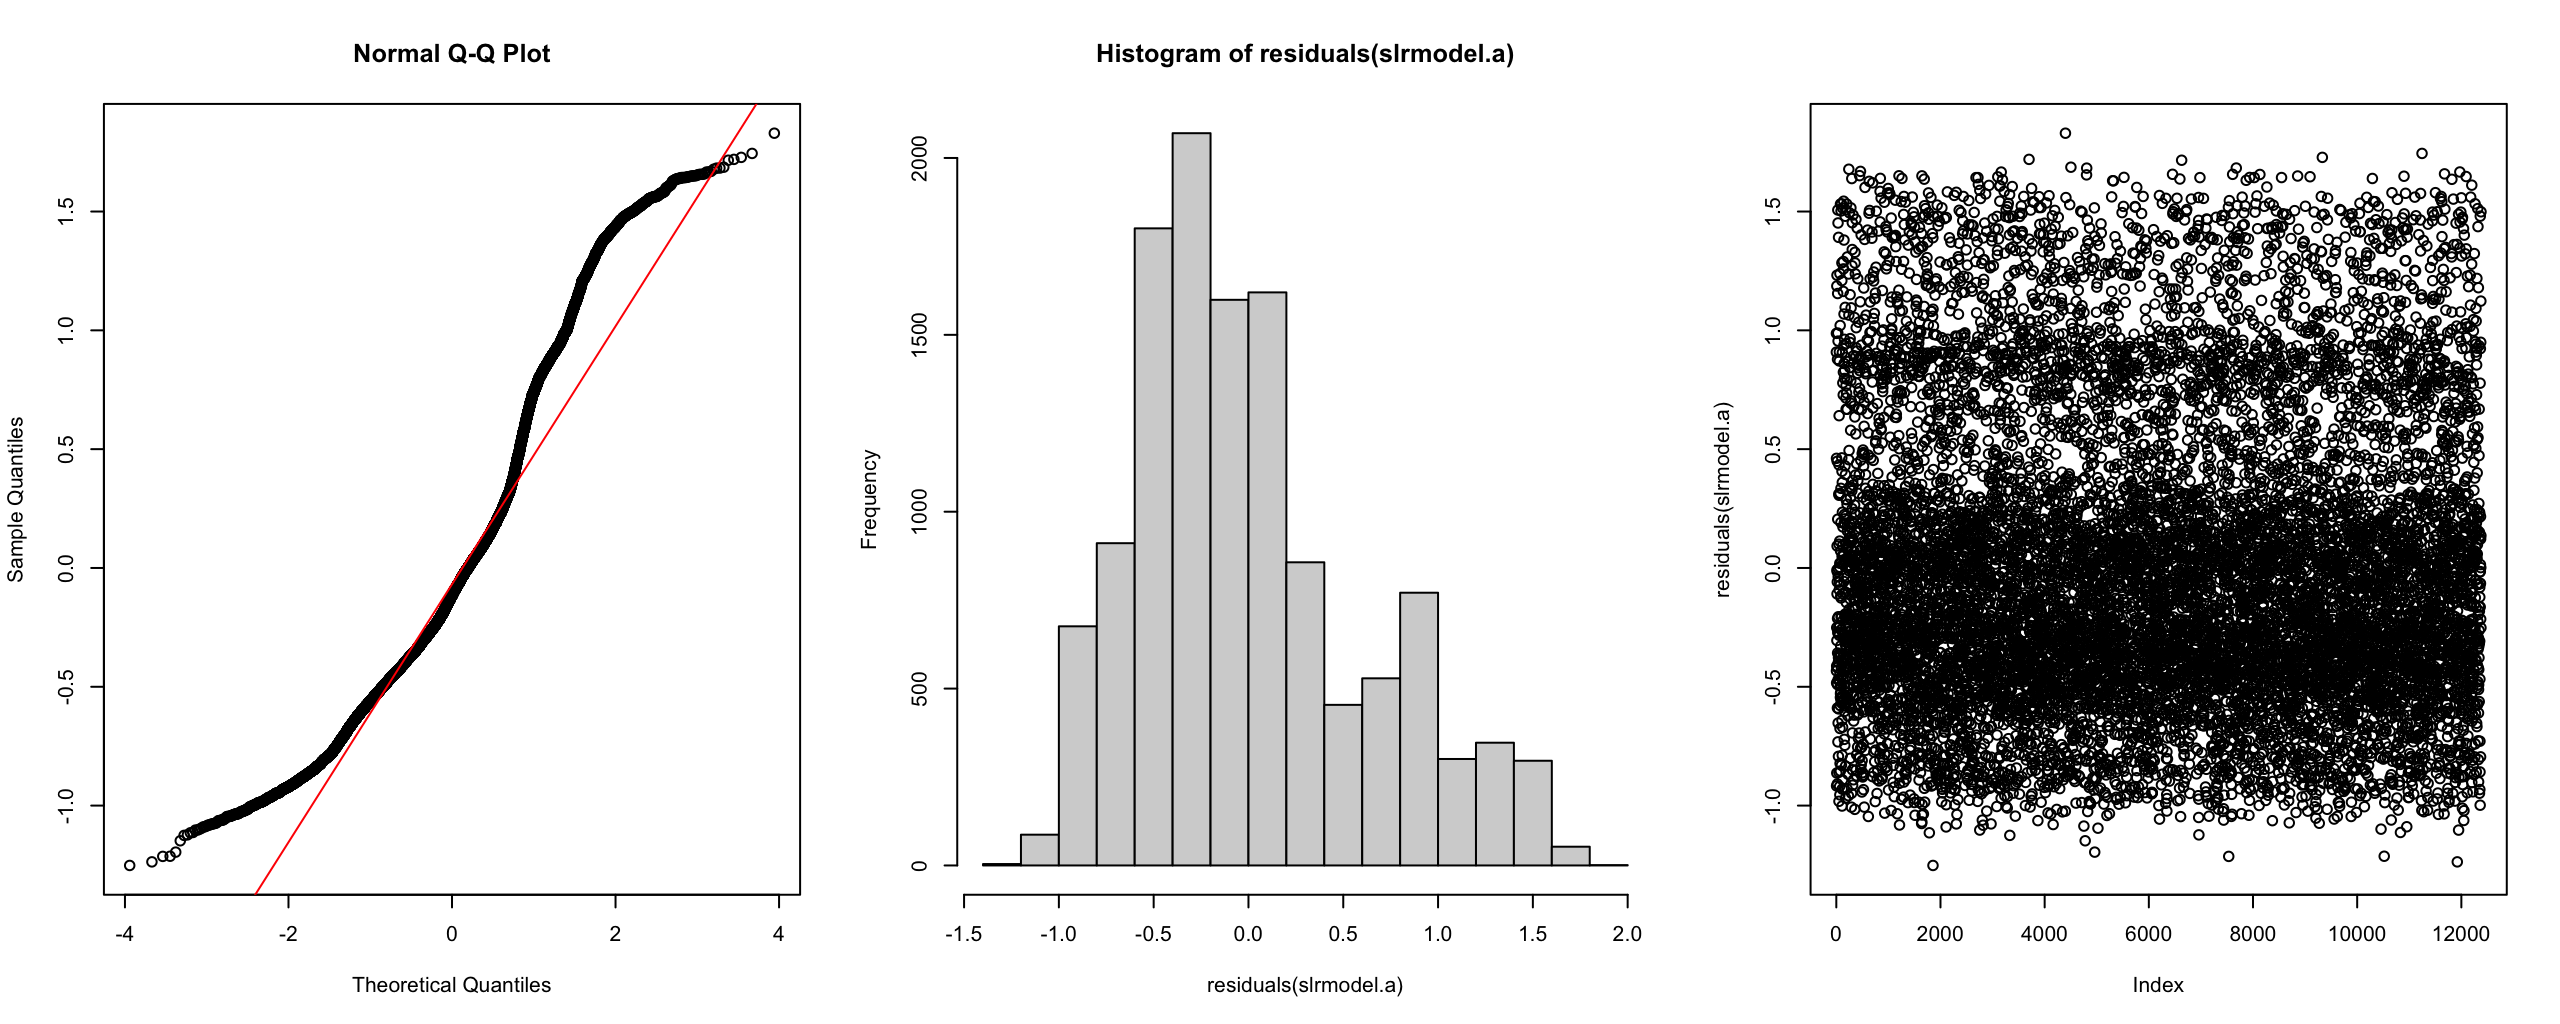
\includegraphics[width=\figsizetext]{Q3/03-reg-assumptions.png}
    \caption{Regression assumptions analysis}
    \label{fig:q3_03}
\end{figure}

This model shows p-value $< 0.05$ on the Breusch-Pagan test, meaning it has signs of heteroscedasticity.

\subsubsection*{Conclusion}

\begin{table}[htbp]
    \centering
    \begin{tabular}{l r r r l}
        \hline
        \multicolumn{5}{l}{\textbf{Residuals}} \\
        Min & 1Q & Median & 3Q & Max \\
        -1.2519 & -0.4347 & -0.1157 & 0.2976 & 1.8296 \\
        \hline
        \textbf{Coefficients} & \textbf{Estimate} & \textbf{Std. Error} & \textbf{t value} & \textbf{Pr($>$$|$t$|$)} \\ 
        \hline
        (Intercept) & 1.113\text{e+}01  & 1.752\text{e-}02 & 635.5  & $< 2\text{e-}16$ *** \\
        RangeKm     & 1.654\text{e-}03  & 5.508\text{e-}06 & 300.4  & $< 2\text{e-}16$ *** \\
        RangeKm\_2  & -7.052\text{e-}08 & 3.023\text{e-}10 & -233.3 & $< 2\text{e-}16$ *** \\
        \hline
        \multicolumn{5}{l}{\textbf{Model Statistics}} \\
        \multicolumn{5}{l}{Residual standard error: 0.6079 on 12374 degrees of freedom} \\
        \multicolumn{5}{l}{Multiple $R^2$: 0.944, \quad Adjusted $R^2$: 0.944} \\
        \multicolumn{5}{l}{F-statistic: $1.043\text{e+}05$ on 2 and 12374 DF, \quad p-value: $< 2.2\text{e-}16$} \\
        \hline
    \end{tabular}
    \caption{Summary of Linear Regression (Model A with Quadratic Term)}
    \label{tab:q3_04}
\end{table}

We selected \texttt{RangeKm} (along with its quadratic transformation) as the best single predictor because it shows a high correlation with Price and explains the highest proportion of the variance in airplane prices. Results reported in table \ref{tab:q3_04}.
\begin{itemize}
    \item \textbf{Intercept ($\beta_0$)}: The expected $\log(\text{Price})$ or baseline price of a plane.
    \item \textbf{Slope for RangeKm ($\beta_1$ \& $\beta_2$)}: For each additional \texttt{RangeKm}, the $\log(\text{Price})$ increases by $\beta_1$ and $\beta_2$, meaning Price increases exponentially by $e^{\beta_2}$.
\end{itemize}

\subsection[Q3-b]{Fit a multivariate linear regression model with the most important two (numerical) variables. Use transformations if it is needed and test all the assumptions. Then compare this model to the simple linear regression model that you fit in (a). Which one is a better model? Why?}

First, we checked a model against all our top variables: \texttt{Capacity}, \texttt{RangeKm}, \texttt{FC}, and \texttt{Age}, table \ref{tab:q3_05}.

\begin{verbatim}
    regmodel.all <- lm(Price ~ ., data = numeric_air_data)
\end{verbatim}

\begin{table}[htbp]
    \centering
    \begin{tabular}{l r r r l}
        \hline
        \multicolumn{5}{l}{\textbf{Residuals}} \\
        Min & 1Q & Median & 3Q & Max \\
        -2.8521 & -0.3464 & 0.1172 & 0.5222 & 1.6157 \\
        \hline
        \textbf{Coefficients} & \textbf{Estimate} & \textbf{Std. Error} & \textbf{t value} & \textbf{Pr($>$$|$t$|$)} \\ 
        \hline
        (Intercept) & 1.682\text{e+}01  & 2.569\text{e-}02 & 654.989  & $< 2\text{e-}16$ *** \\
        Capacity    & 3.080\text{e-}02  & 3.505\text{e-}04 & 87.856   & $< 2\text{e-}16$ *** \\
        RangeKm     & -4.671\text{e-}04 & 8.884\text{e-}06 & -52.576  & $< 2\text{e-}16$ *** \\
        FC          & -8.760\text{e-}02 & 8.055\text{e-}04 & -108.751 & $< 2\text{e-}16$ *** \\
        HM          & 2.249\text{e-}06  & 5.190\text{e-}06 & 0.433    & 0.665 \\
        Age         & -1.819\text{e-}02 & 5.258\text{e-}04 & -34.590  & $< 2\text{e-}16$ *** \\
        \hline
        \multicolumn{5}{l}{\textbf{Model Statistics}} \\
        \multicolumn{5}{l}{Residual standard error: 0.7465 on 12371 degrees of freedom} \\
        \multicolumn{5}{l}{Multiple $R^2$: 0.9156, \quad Adjusted $R^2$: 0.9155} \\
        \multicolumn{5}{l}{F-statistic: $2.683\text{e+}04$ on 5 and 12371 DF, \quad p-value: $< 2.2\text{e-}16$} \\
        \hline
    \end{tabular}
    \caption{Summary of Multiple Linear Regression (All Predictors)}
    \label{tab:q3_05}
\end{table}


\begin{verbatim}
    regmodel.best4 <- lm(Price ~ Capacity + RangeKm + FC + Age, data = numeric_air_data)
    
    anova(regmodel.all, regmodel.best4)
\end{verbatim}

The ANOVA confirmed that the model with all predictors is not significantly better than the model with these 4 predictors. However, checking Variance Inflation Factors (VIF) revealed critical multicollinearity (tables \ref{tab:q3_06_vif} and \ref{tab:q3_06_cor}).

\begin{verbatim}
    cor(numeric_air_data[,-price.col])
    vif(regmodel.best4)
\end{verbatim}
\begin{table}[htbp]
  \centering
  \caption{Correlation Matrix for Numeric Variables}
  \begin{tabular}{lrrrrr}
    \toprule
    & \textbf{Capacity} & \textbf{RangeKm} & \textbf{FC} & \textbf{HM} & \textbf{Age} \\
    \midrule
    Capacity &  1.000 &  0.990 & -0.468 & -0.012 &  0.019 \\
    RangeKm  &  0.990 &  1.000 & -0.424 & -0.014 &  0.019 \\
    FC       & -0.468 & -0.424 &  1.000 & -0.011 & -0.020 \\
    HM       & -0.012 & -0.014 & -0.011 &  1.000 &  0.010 \\
    Age      &  0.019 &  0.019 & -0.020 &  0.010 &  1.000 \\
    \bottomrule
  \end{tabular}
  \label{tab:q3_06_cor}
\end{table}

\begin{table}[htbp]
  \centering
  \caption{Variance Inflation Factors for Best 4 Model}
  \begin{tabular}{lr}
    \toprule
    \textbf{Predictor Variable} & \textbf{VIF}   \\
    \midrule
    Capacity                   & 55.540733      \\
    RangeKm                    & 52.879523      \\
    FC                         & 1.413722       \\
    Age                        & 1.000534       \\
    \bottomrule
  \end{tabular}
  \label{tab:q3_06_vif}
\end{table}

The Correlation Matrix and VIF tell us that Capacity and RangeKm are highly correlated. VIF also tell us that there is a multicollinearity problem within our predictors. We choose to drop the predictor with the highest VIF: \texttt{Capacity}.

Now, VIF shows no multicollinearity among the selected predictors.

By systematically dropping predictors and comparing via ANOVA, we discovered that keeping \texttt{RangeKm} and \texttt{FC} led to higher $R^2$ and a smaller Sum of Square Residuals. Similar to the SLR, adding a quadratic term $\texttt{RangeKm}^2$ further improved the model.

\subsubsection*{Model A vs Model B comparison}

\begin{table}[htbp]
    \centering
    \begin{tabular}{l r r r r r l}
        \hline
        \multicolumn{7}{l}{\textbf{Model 1:} Price $\sim$ RangeKm + RangeKm\_2} \\
        \multicolumn{7}{l}{\textbf{Model 2:} Price $\sim$ RangeKm\_2 + RangeKm + FC} \\
        \hline
          & \textbf{Res.Df} & \textbf{RSS} & \textbf{Df} & \textbf{Sum of Sq} & \textbf{F} & \textbf{Pr($>$F)} \\ 
        \hline
        1 & 12374 & 4572.8 &   &        &        & \\
        2 & 12373 & 3321.5 & 1 & 1251.3 & 4661.3 & $< 2.2\text{e-}16$ *** \\
        \hline
    \end{tabular}
    \caption{Analysis of Variance Table: Model A vs Model B}
    \label{tab:q3_07}
\end{table}

\begin{itemize}
    \item The MLR model with \texttt{RangeKm} + $\texttt{RangeKm}^2$ + \texttt{FC} has a higher adjusted $R^2$ and a lower residual standard error than the SLR with Capacity alone, indicating a better fit.
    \item The ANOVA F-test confirms that adding the second variable significantly improves the model.
\end{itemize}

The assumptions can be visualized in figure \ref{fig:q3_08}.

\begin{figure}[htbp]
    \centering
    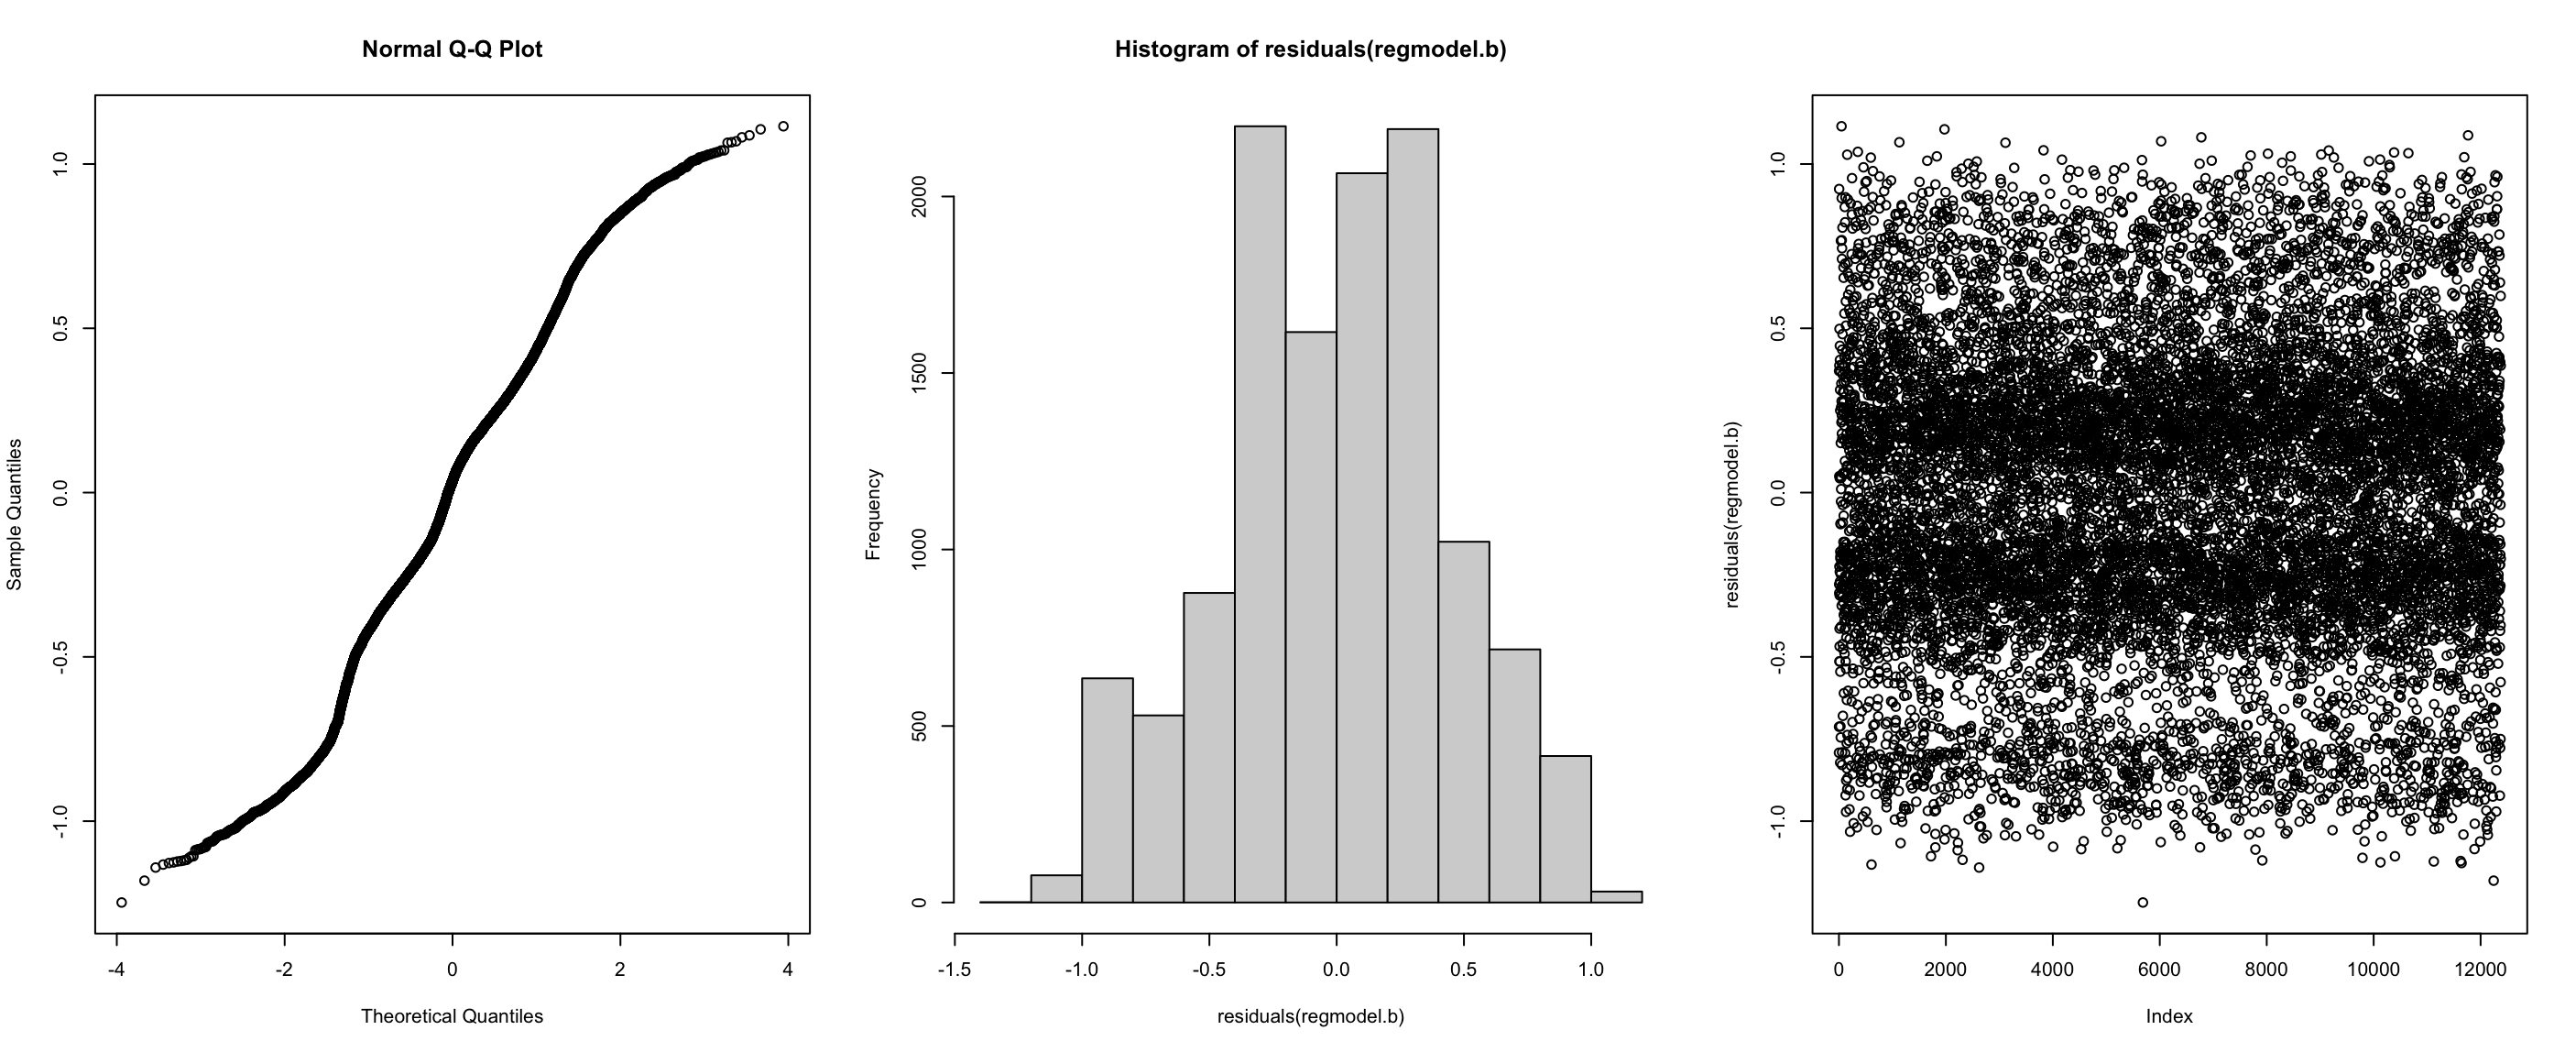
\includegraphics[width=\figsizetext]{Q3/08-modelb-assumptions.png}
    \caption{Assumptions analysis for Model B}
    \label{fig:q3_08}
\end{figure}

\subsection[Q3-c]{Encode the variable model into three categories considering whether the plane is ``Airbus'', ``Boeing'' or ``Other''. Now add this model factor to the regression model you have chosen in subsection (b). Interpret the coefficients and overall summary of the model. Compare the model in subsection (b) with the model that has an additional factor. Which one would you choose? Why?}

We added \texttt{ModelCat} to our selected model. However, introducing \texttt{ModelCat} made \texttt{FC} statistically insignificant. We dropped \texttt{FC} to simplify the model, yielding: \texttt{lm(Price \textasciitilde{} RangeKm\_2 * ModelCat + RangeKm)}. lm result is reported in table \ref{tab:q3_09}, while the residuals are in figure \ref{fig:q3_10}.

\begin{table}[htbp]
    \centering
    \begin{tabular}{l r r r l}
        \hline
        \multicolumn{5}{l}{\textbf{Residuals}} \\
        Min & 1Q & Median & 3Q & Max \\
        -0.62176 & -0.21716 & -0.07364 & 0.22958 & 0.75755 \\
        \hline
        \textbf{Coefficients} & \textbf{Estimate} & \textbf{Std. Error} & \textbf{t value} & \textbf{Pr($>$$|$t$|$)} \\ 
        \hline
        (Intercept)               &  5.233\text{e+}00 & 2.792\text{e-}02 &  187.46 & $< 2\text{e-}16$ *** \\
        RangeKm\_2                & -1.288\text{e-}07 & 2.970\text{e-}10 & -433.75 & $< 2\text{e-}16$ *** \\
        ModelCatBoeing            &  5.520\text{e-}01 & 1.009\text{e-}02 &   54.69 & $< 2\text{e-}16$ *** \\
        ModelCatOther             &  3.755\text{e+}00 & 1.741\text{e-}02 &  215.72 & $< 2\text{e-}16$ *** \\
        RangeKm                   &  2.901\text{e-}03 & 6.150\text{e-}06 &  471.76 & $< 2\text{e-}16$ *** \\
        RangeKm\_2:ModelCatBoeing &  1.332\text{e-}09 & 6.122\text{e-}11 &   21.76 & $< 2\text{e-}16$ *** \\
        RangeKm\_2:ModelCatOther  &  NA               & NA               &  NA     & NA \\
        \hline
        \multicolumn{5}{l}{\textbf{Model Statistics}} \\
        \multicolumn{5}{l}{Residual standard error: 0.2686 on 12371 degrees of freedom} \\
        \multicolumn{5}{l}{Multiple $R^2$: 0.9891, \quad Adjusted $R^2$: 0.9891} \\
        \multicolumn{5}{l}{F-statistic: $2.24\text{e+}05$ on 5 and 12371 DF, \quad p-value: $< 2.2\text{e-}16$} \\
        \hline
    \end{tabular}
    \caption{Summary of Multiple Linear Regression (Model C Interaction)}
    \label{tab:q3_09}
\end{table}

\subsubsection*{Interpretation}
\begin{itemize}
    \item \textbf{Intercept ($\beta_0$)}: Expected $\log(\text{Price})$ for the baseline category.
    \item \textbf{ModelCat effects}: The coefficients for Boeing and ``Other'' represent the shift in the baseline $\log(\text{Price})$ compared to Airbus.
    \item \textbf{Interaction ($\texttt{RangeKm\_2} \times \texttt{ModelCat}$)}: The slope for the squared range changes depending on the airplane manufacturer.
\end{itemize}

\begin{figure}[htbp]
    \centering
    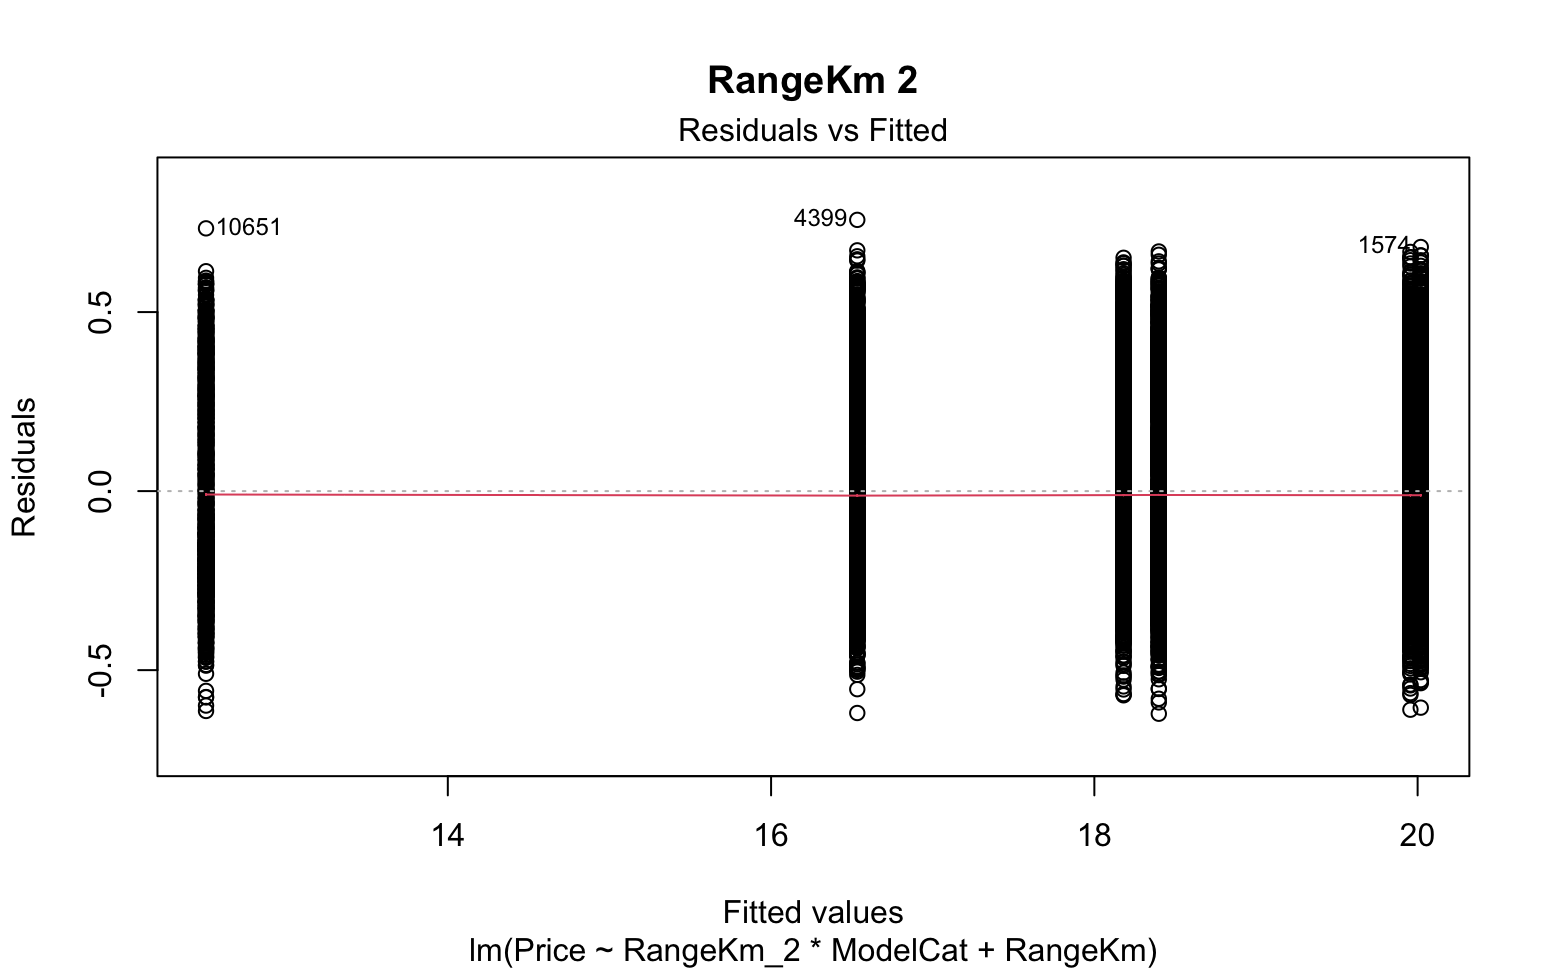
\includegraphics[width=\figsizetext]{Q3/10-modelc-res-vs-fitted.png}
    \caption{Residual vs Fitted for Model C}
    \label{fig:q3_10}
\end{figure}

The Residual vs Fitted plot shows good results.

\subsubsection*{Model B vs Model C comparison}

\begin{table}[htbp]
    \centering
    \begin{tabular}{l r r r r r l}
        \hline
        \multicolumn{7}{l}{\textbf{Model 1:} Price $\sim$ RangeKm\_2 + RangeKm + FC} \\
        \multicolumn{7}{l}{\textbf{Model 2:} Price $\sim$ RangeKm\_2 * ModelCat + RangeKm + FC} \\
        \hline
          & \textbf{Res.Df} & \textbf{RSS} & \textbf{Df} & \textbf{Sum of Sq} & \textbf{F} & \textbf{Pr($>$F)} \\ 
        \hline
        1 & 12373 & 3321.5 &   &        &       & \\
        2 & 12370 &  892.2 & 3 & 2429.3 & 11227 & $< 2.2\text{e-}16$ *** \\
        \hline
    \end{tabular}
    \caption{Analysis of Variance Table: Model B vs Model C}
    \label{tab:q3_11}
\end{table}

\begin{itemize}
    \item The ANOVA analysis tells us that adding \texttt{ModelCat} decreases the Residual Sum of Squares, meaning the model significantly improves with this new variable.
    \item We selected this interaction model (Model C) as our best model.
\end{itemize}

\subsection[Q3-d]{Test the validity of the final model that you choose.}

\begin{figure}[htbp]
    \centering
    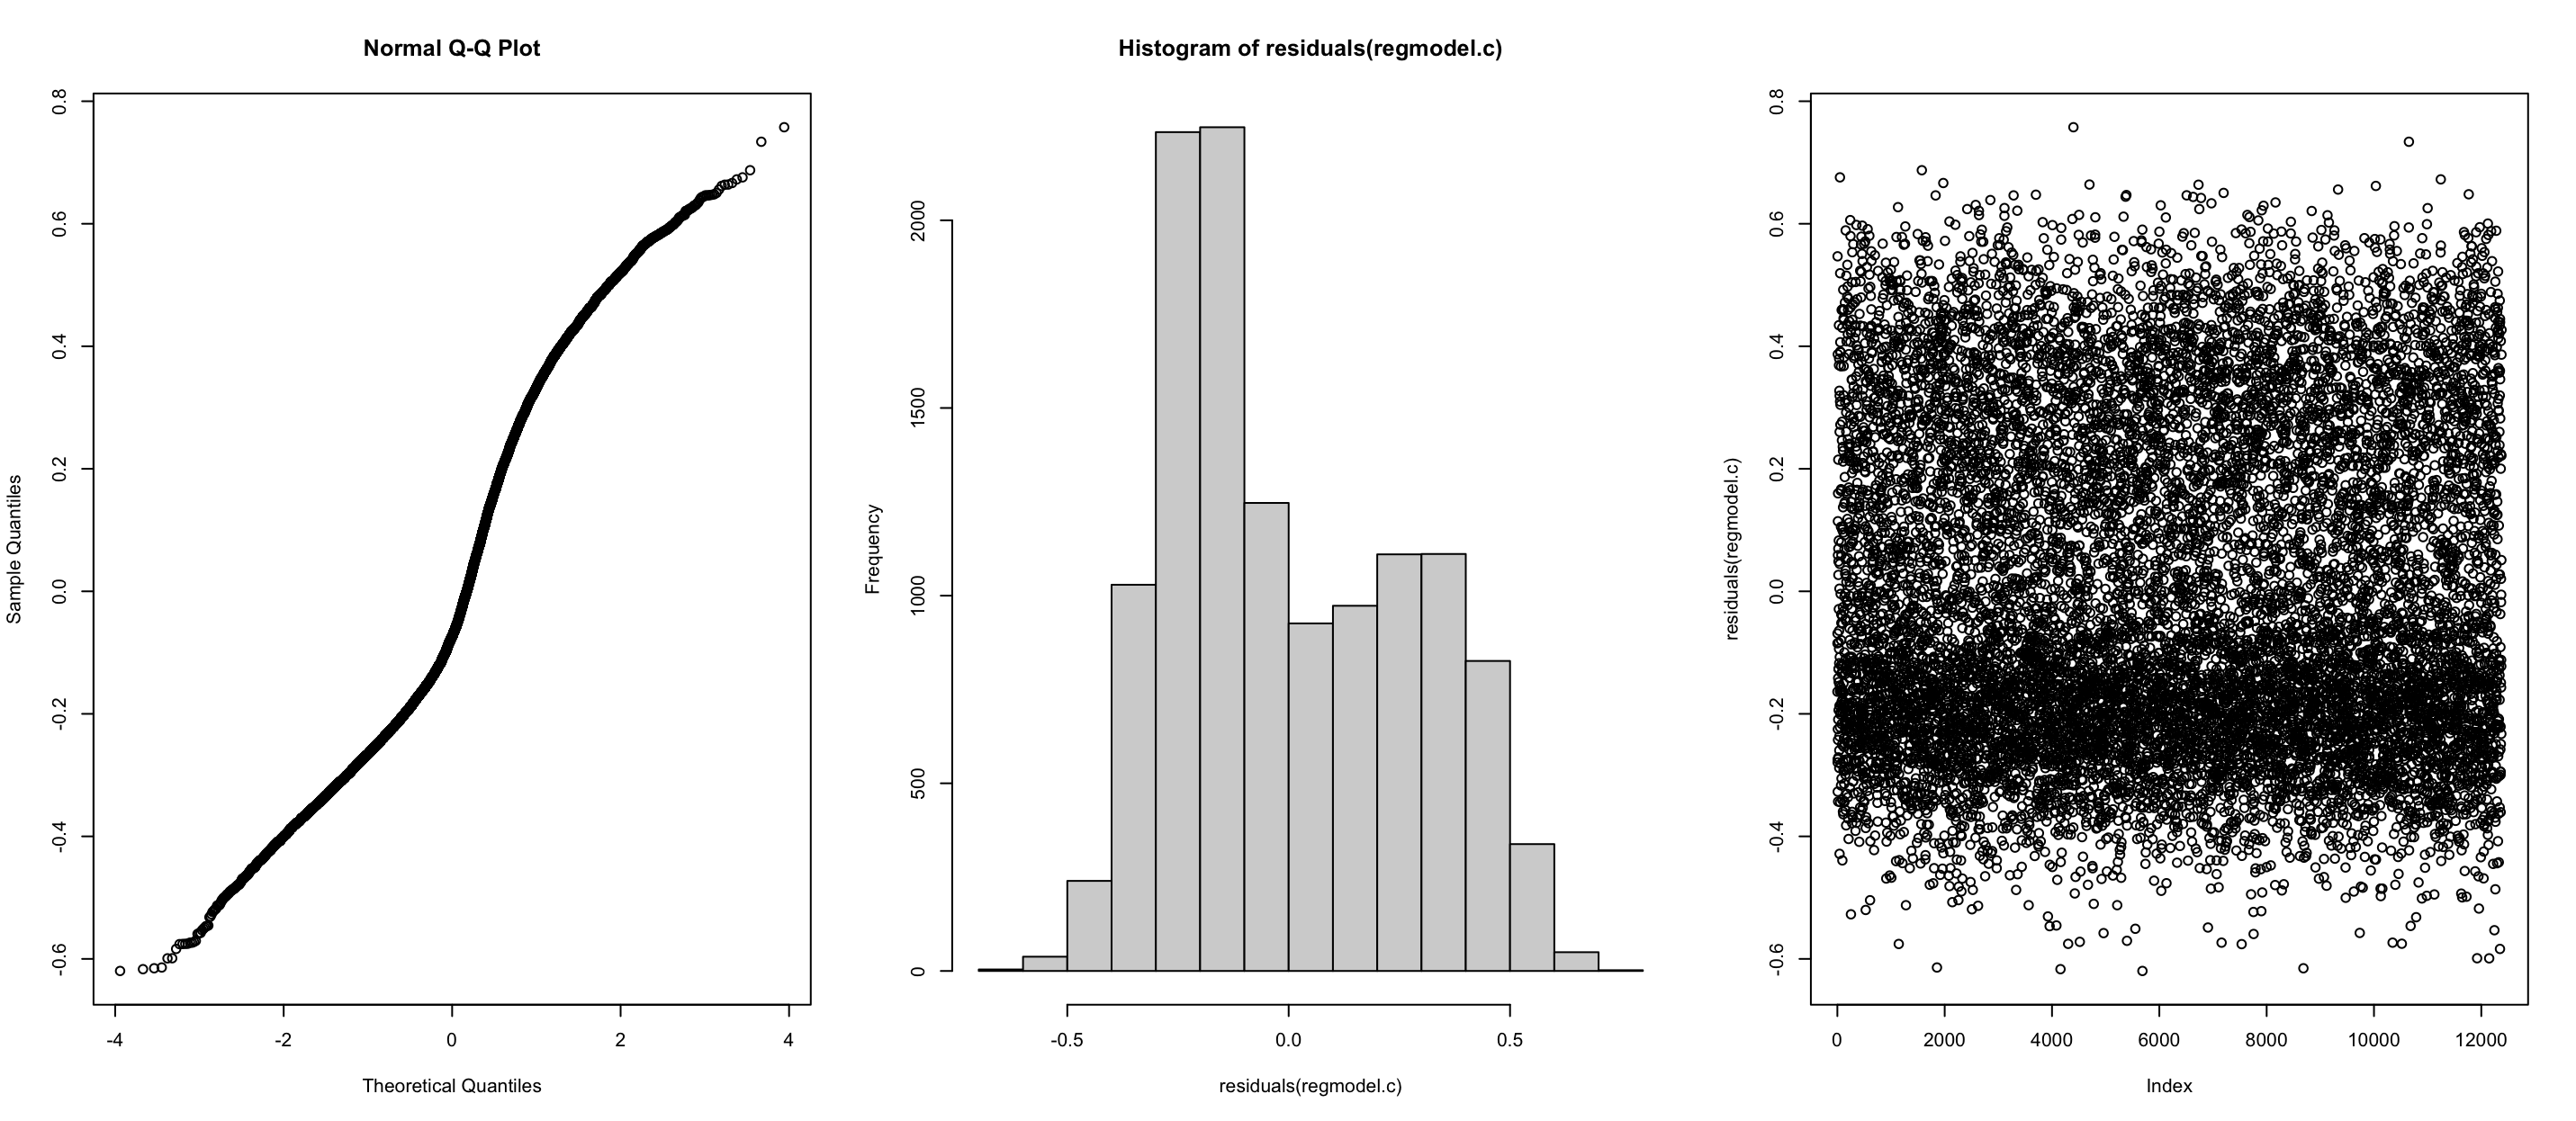
\includegraphics[width=\figsizetext]{Q3/12-modelc-assumptions.png}
    \caption{Validity test for final model C}
    \label{fig:q3_12}
\end{figure}

To fully validate the predictive power of our chosen model (\texttt{Price \textasciitilde{} RangeKm\_2 * ModelCat + RangeKm}), we split the data into an 80\% training set and a 20\% testing set.


\subsubsection*{Validity and Performance}
\begin{itemize}
    \item \textbf{Out-of-sample MSE}: We calculated the Mean Squared Error against the holdout Test Set, which quantifies the average squared prediction error on unseen data.
    \item \textbf{Diagnostics}: The Q-Q plot of the final model mostly follows the diagonal (normality holds). Durbin-Watson statistic is close to 2 (no autocorrelation).
    \item Plotting \texttt{Actual vs Predicted} (figure \ref{fig:q3_13}) values from the test set showed data points clustering closely around the ideal $y = x$ reference line, meaning the model generalizes well and confirms our findings.
\end{itemize}
\begin{figure}[htbp]
    \centering
    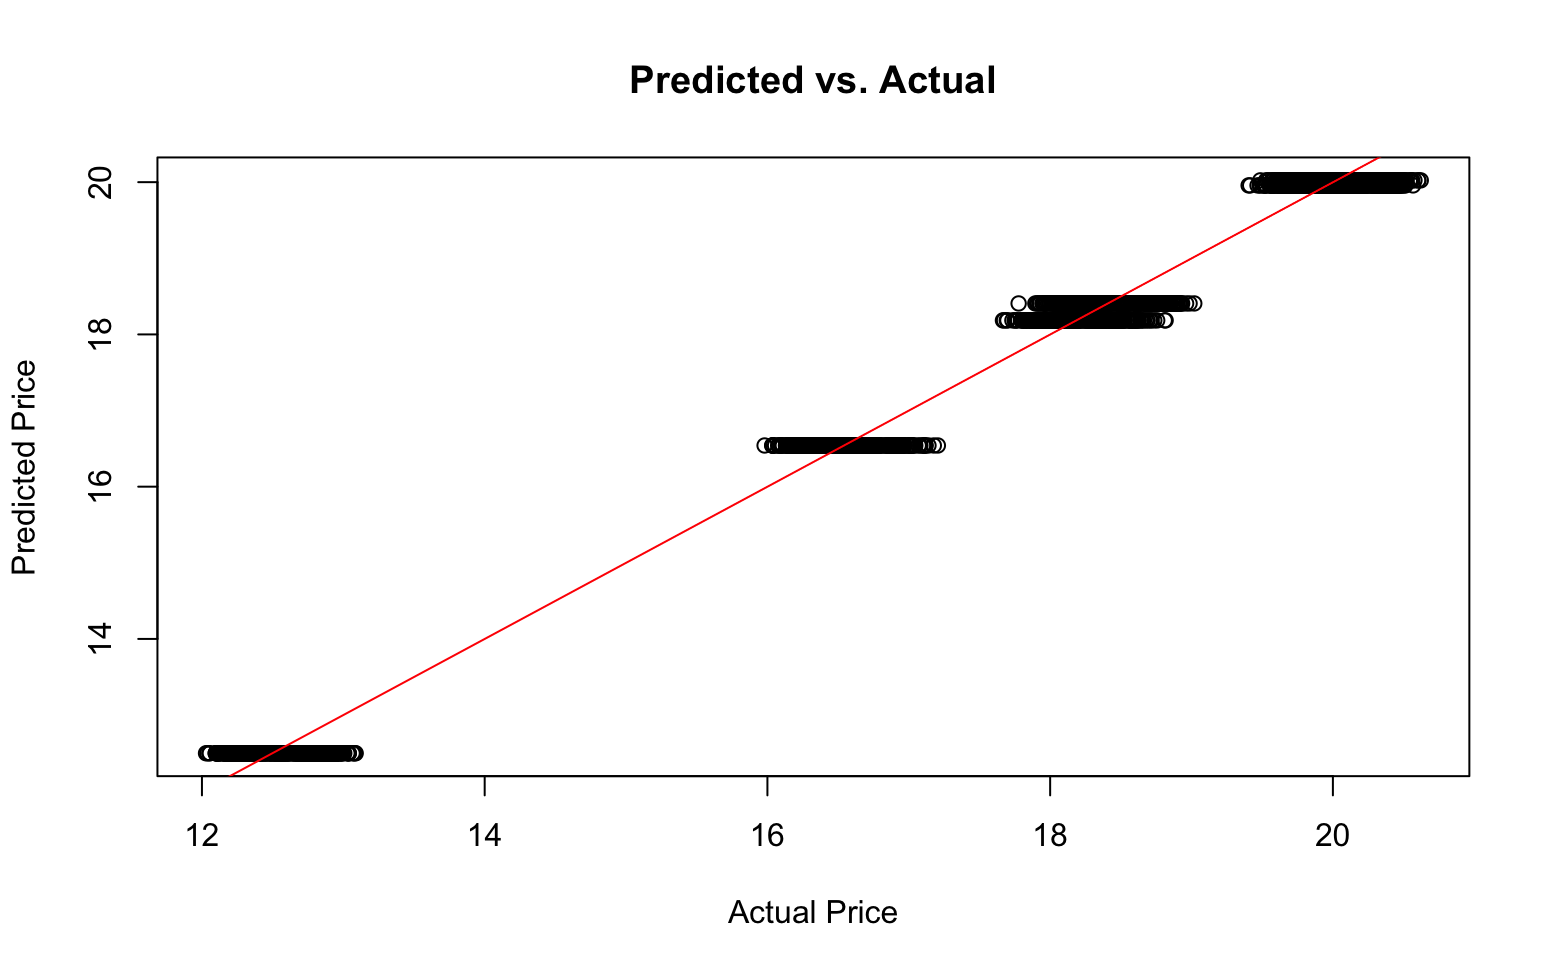
\includegraphics[width=\figsizetext]{Q3/13-actual-vs-predicted.png}
    \caption{Actual vs Predicted values}
    \label{fig:q3_13}
\end{figure}